\documentclass[11pt]{article}
\usepackage[utf8]{inputenc}
\usepackage{authblk}
\usepackage{graphicx}
\usepackage{amsmath,amssymb}
\usepackage{hyperref}
\usepackage{booktabs}
\usepackage{multirow}
\usepackage{xcolor}
\usepackage{algorithm}
\usepackage{algpseudocode}
\usepackage{tikz}
\usetikzlibrary{shapes,arrows,positioning,fit,backgrounds}
\usepackage{geometry}
\geometry{margin=1in}
\usepackage{enumitem}
\setlist{nosep}

\title{Improving Operation Accuracy in Computer Use Agents by Adopting Semantic Knowledge: A Comprehensive Survey}
\author[1]{Guang Yang}
\affil[1]{Department of Computer Science}
\date{February 2026}

\begin{document}
\maketitle

\begin{abstract}
Graphical user interfaces (GUIs) present a formidable challenge for artificial agents because they require the integration of visual perception, natural language understanding, semantic reasoning, and sequential action planning. Contemporary agents based on multimodal large language models (MLLMs) interleave vision and text encoders but often misinterpret icons, misjudge system states, hallucinate non-existent actions, or fail to generalize across applications. Humans achieve robust interaction by leveraging rich \textit{world knowledge}: we infer three-dimensional layouts from two-dimensional projections, recognize polysemous icons through accumulated experience, and interpret interface semantics via linguistic and cultural context. This survey synthesizes research on how general and semantic knowledge can dramatically improve the reliability and accuracy of GUI-based computer use agents. We provide a comprehensive review spanning: (1) cognitive science foundations of human world understanding and icon comprehension; (2) vision encoders and their role in UI perception; (3) text encoders and linguistic knowledge for instruction understanding; (4) knowledge graphs and structured semantic reasoning; (5) multimodal fusion architectures that combine these components; (6) benchmarks and datasets that expose knowledge gaps in current models; and (7) state-of-the-art GUI agents and their architectures. We analyze the critical \textit{knowledge--action gap} that limits current systems and propose a unified framework for knowledge-augmented GUI agents. Finally, we outline promising research directions including imbalanced representation learning, prototype-based relation modeling, and dynamic knowledge graph integration.
\end{abstract}

\section{Introduction}
\label{sec:intro}

The automation of graphical user interfaces represents one of the most practical yet challenging frontiers in artificial intelligence. Unlike structured APIs or command-line interfaces, GUIs are designed for human visual perception and manual interaction, presenting agents with pixel-level inputs that must be interpreted through the lens of visual understanding, semantic reasoning, and procedural knowledge.

\subsection{The Human Advantage}

Humans effortlessly operate complex software by leveraging high-level understanding of the physical world and cultural conventions. When we first encounter an unfamiliar application, we draw upon multiple knowledge sources:

\begin{itemize}
    \item \textbf{Visual-spatial knowledge}: We perceive depth, layout, and grouping from 2D renderings, inferring which elements are interactive and how they relate spatially.
    \item \textbf{Semantic knowledge}: We recognize that a trash can icon typically represents deletion, a floppy disk suggests saving, and a gear indicates settings---regardless of specific visual rendering.
    \item \textbf{Procedural knowledge}: We understand that complex tasks decompose into sequences of atomic actions, with dependencies and prerequisites.
    \item \textbf{Linguistic knowledge}: We parse button labels, menu items, and tooltips using natural language understanding, handling synonyms, abbreviations, and domain-specific terminology.
\end{itemize}

This rich integration of knowledge sources enables humans to transfer skills across applications, recover from errors, and accomplish novel tasks with minimal instruction. Current AI agents largely lack this capability.

\subsection{The Knowledge--Action Gap}

Despite remarkable advances in large language models (LLMs) and vision-language models (VLMs), GUI agents exhibit a persistent \textit{knowledge--action gap}: they may possess relevant knowledge yet fail to translate it into correct actions. Studies on the OSWorld benchmark~\cite{osworld2024} demonstrate that even when agents retrieve task instructions that are 90\% correct, they achieve only a 41\% success rate. This gap manifests in several ways:

\begin{enumerate}
    \item \textbf{Perception failures}: Agents misidentify UI elements, confuse similar icons, or fail to detect elements in non-standard locations.
    \item \textbf{State tracking failures}: Agents lose track of application state across interaction steps, leading to redundant or contradictory actions.
    \item \textbf{Planning failures}: Agents cannot decompose complex tasks into correct action sequences or recover from execution errors.
    \item \textbf{Grounding failures}: Agents generate actions that reference non-existent elements or use incorrect coordinates.
\end{enumerate}

\subsection{Thesis and Contributions}

This survey argues that \textbf{injecting general and semantic knowledge into GUI agents---through vision encoders, text encoders, knowledge graphs, and linguistic resources---can dramatically improve operation accuracy}. We make the following contributions:

\begin{enumerate}
    \item We provide a comprehensive taxonomy of knowledge types relevant to GUI understanding, grounded in cognitive science research on human perception and learning.
    \item We systematically review vision encoder architectures for UI perception, including CNN-based, ViT-based, and hybrid approaches.
    \item We analyze text encoders and linguistic knowledge sources that enable instruction understanding and cross-lingual transfer.
    \item We survey knowledge graph construction and integration methods for structured semantic reasoning.
    \item We examine multimodal fusion architectures that combine vision, language, and structured knowledge.
    \item We provide an extensive review of benchmarks, datasets, and evaluation protocols that reveal knowledge gaps.
    \item We analyze state-of-the-art GUI agents and propose a unified framework for knowledge-augmented computer use.
    \item We outline promising research directions including imbalanced representation learning, prototype-based reasoning, and dynamic knowledge evolution.
\end{enumerate}

\subsection{Survey Organization}

The remainder of this survey is organized as follows. Section~\ref{sec:cognitive} reviews cognitive science foundations of human world understanding and icon comprehension. Section~\ref{sec:vision} examines vision encoders for UI perception. Section~\ref{sec:text} covers text encoders and linguistic knowledge. Section~\ref{sec:kg} surveys knowledge graphs and structured reasoning. Section~\ref{sec:fusion} analyzes multimodal fusion architectures. Section~\ref{sec:benchmarks} reviews benchmarks and datasets. Section~\ref{sec:agents} examines state-of-the-art GUI agents. Section~\ref{sec:framework} proposes a unified framework. Section~\ref{sec:future} outlines future directions, and Section~\ref{sec:conclusion} concludes.

\section{Cognitive Foundations of World Knowledge}
\label{sec:cognitive}

Understanding how humans perceive and interact with interfaces provides essential foundations for designing knowledge-aware agents. We review cognitive research on 3D perception, icon comprehension, and semantic memory.

\subsection{Constructing Three-Dimensional Representations}

Humans do not perceive the world as a collage of flat images. Developmental psychology demonstrates that infants as young as two months use motion cues to extract 3D structure~\cite{slater1985}, and volumetric completion emerges between four and six months~\cite{soska2010}. In a classic habituation study, 4- and 6-month-old infants were shown a rotating wedge; only the older infants preferred the novel incomplete display, suggesting they represented the wedge as a complete 3D volume.

Adults likewise infer depth from parallax, shading, occlusion, and perspective cues. When first viewing multiple overlapping windows on a screen, we immediately perceive a depth ordering despite the 2D pixel representation. This inferential process---constructing 3D mental models from 2D projections---underlies our ability to navigate interfaces where icons, windows, and dialogs exist in a conceptual depth hierarchy.

\textbf{Implications for agents}: GUI agents should develop internal representations that capture spatial relationships beyond pixel coordinates, including containment, overlap, and depth ordering. Current vision encoders largely ignore these relationships.

\subsection{Knowledge Sources for Icon Comprehension}

Icons are inherently ambiguous visual symbols. A printer icon could represent printing a document, configuring print settings, accessing the print queue, or even a device status indicator. Dessus and Peraya~\cite{dessus2000} identify seven knowledge sources that humans integrate for icon comprehension:

\begin{enumerate}
    \item \textbf{Domain knowledge}: Understanding of the task domain (e.g., document editing, image manipulation).
    \item \textbf{System knowledge}: Familiarity with the specific application and its conventions.
    \item \textbf{Work context knowledge}: Understanding of the non-computerized version of the task.
    \item \textbf{Problem knowledge}: Awareness of the current goal and constraints.
    \item \textbf{Operational knowledge}: Knowledge of how to execute system commands.
    \item \textbf{Natural language knowledge}: Ability to interpret labels, tooltips, and menus.
    \item \textbf{Device knowledge}: Familiarity with input devices (mouse, keyboard, touch).
\end{enumerate}

Semantic memory---the repository of general world knowledge---significantly enhances icon recognition. Recognition is faster and more accurate when icons are semantically meaningful, suggesting that meaning provides top-down facilitation of perception~\cite{iconcomplex2020}.

\textbf{Implications for agents}: Effective GUI agents must integrate multiple knowledge sources, not just visual pattern matching. This motivates architectures that combine vision encoders with knowledge graphs and language models.

\subsection{Cognitive Load and Interface Learning}

Cognitive load theory~\cite{sweller1988} explains how working memory limitations affect learning and performance. When interacting with novel interfaces, humans experience \textit{intrinsic load} (task complexity), \textit{extraneous load} (interface complexity), and \textit{germane load} (learning effort). Well-designed interfaces and effective prior knowledge reduce extraneous load, freeing cognitive resources for task completion.

Experts exhibit \textit{chunking}---organizing interface elements into meaningful units based on prior knowledge. A document editor user perceives the formatting toolbar as a coherent unit rather than individual buttons. This chunking reduces cognitive load and enables rapid action selection.

\textbf{Implications for agents}: Agents should learn hierarchical representations of interface elements, grouping related components. Attention mechanisms in transformers can model these relationships, but require training signals that encourage semantic grouping.

\section{Vision Encoders for UI Perception}
\label{sec:vision}

Vision encoders transform raw pixel inputs into representations suitable for downstream reasoning. We review architectures specifically designed or adapted for UI understanding.

\subsection{Convolutional Neural Networks}

Early approaches to UI understanding employed convolutional neural networks (CNNs) trained on labeled UI datasets. The RICO dataset~\cite{rico2017} enabled training object detectors for UI components such as buttons, text fields, and images. CNN-based approaches achieve good performance on element detection but struggle with:

\begin{itemize}
    \item \textbf{Resolution limitations}: Standard CNNs downsample inputs, losing fine-grained details critical for text recognition.
    \item \textbf{Fixed receptive fields}: CNNs cannot easily capture long-range dependencies between distant UI elements.
    \item \textbf{Limited semantic understanding}: Pure CNN features lack explicit semantic content.
\end{itemize}

\subsection{Vision Transformers}

Vision Transformers (ViT)~\cite{dosovitskiy2020} divide images into patches and process them through self-attention layers, enabling:

\begin{itemize}
    \item \textbf{Global context}: Self-attention captures relationships between any pair of patches.
    \item \textbf{Scalable resolution}: Larger images require more patches but the architecture remains unchanged.
    \item \textbf{Pretraining transfer}: ViTs pretrained on large image datasets transfer well to UI understanding.
\end{itemize}

However, standard ViTs still face challenges with UI screenshots:

\begin{itemize}
    \item \textbf{Resolution constraints}: High-resolution screenshots may require thousands of patches, exceeding typical context lengths.
    \item \textbf{Text recognition}: While ViTs can encode text regions, they do not explicitly perform OCR.
    \item \textbf{Element granularity}: Patch boundaries may not align with UI element boundaries.
\end{itemize}

\subsection{High-Resolution Vision Encoders}

Modern GUI agents employ high-resolution vision encoders to preserve fine details. CogAgent~\cite{cogagent2023} introduces a dual encoder architecture:

\begin{itemize}
    \item A \textbf{low-resolution encoder} processes downsampled images (224$\times$224) for global context.
    \item A \textbf{high-resolution encoder} processes the original image (1120$\times$1120) through a cross-attention mechanism.
\end{itemize}

This approach captures both global layout and fine-grained details such as small icons and text. CogAgent achieves state-of-the-art performance on GUI navigation tasks while maintaining compatibility with pretrained VLMs.

\subsection{OCR-Enhanced Encoders}

Accurate text recognition is crucial for UI understanding. OmniParser~\cite{omniparser2024} combines:

\begin{itemize}
    \item An \textbf{icon detection model} that localizes interactive elements.
    \item An \textbf{OCR module} that extracts text from screenshots.
    \item A \textbf{captioning model} that generates semantic descriptions of elements.
\end{itemize}

Experiments show that adding OmniParser's structured output to prompts improves GPT-4V's element assignment accuracy from 0.705 to 0.938, demonstrating the value of explicit text extraction.

\subsection{Graph-Based Visual Representations}

ShowUI~\cite{showui2024} treats screenshots as graphs where patches are nodes connected by spatial adjacency. A UI-guided visual token selection scheme identifies tokens corresponding to interactive regions:

\begin{enumerate}
    \item Construct a connectivity graph over image patches.
    \item Identify connected components likely to contain UI elements.
    \item Select representative tokens from each component.
\end{enumerate}

This approach reduces redundant tokens by 33\% and accelerates training by 1.4$\times$ while achieving 75.1\% zero-shot grounding accuracy.

\subsection{Multi-Scale Feature Extraction}

UI elements span multiple scales---from small icons to large content areas. Feature pyramid networks (FPN) and multi-scale attention mechanisms address this challenge:

\begin{itemize}
    \item \textbf{FPN adapters}: Insert feature pyramid layers after pretrained encoders to capture multi-scale features.
    \item \textbf{Multi-scale attention}: Compute attention at multiple resolutions and fuse results.
    \item \textbf{Deformable attention}: Attend to learned sparse locations rather than all patches.
\end{itemize}

\section{Text Encoders and Linguistic Knowledge}
\label{sec:text}

Text encoders process natural language instructions and generate semantic representations for action selection. We review encoder architectures and linguistic knowledge sources.

\subsection{Transformer-Based Language Models}

Modern GUI agents employ transformer-based language models for instruction understanding and action generation. Key architectures include:

\begin{itemize}
    \item \textbf{Encoder-only models} (BERT, RoBERTa): Produce contextual embeddings for classification and matching.
    \item \textbf{Decoder-only models} (GPT series): Generate action sequences autoregressively.
    \item \textbf{Encoder-decoder models} (T5, BART): Transform instructions into structured outputs.
\end{itemize}

For GUI agents, decoder-only architectures dominate because they naturally generate action sequences and integrate well with reinforcement learning.

\subsection{Instruction Understanding}

GUI agents must parse diverse instruction formats:

\begin{itemize}
    \item \textbf{Imperative commands}: ``Click the save button'', ``Open settings''.
    \item \textbf{Goal descriptions}: ``I want to print this document'', ``Make the text bold''.
    \item \textbf{Conditional requests}: ``If there's an error, click OK''.
    \item \textbf{Multi-step procedures}: ``First open File menu, then click Export, and select PDF''.
\end{itemize}

Large language models excel at instruction understanding through pretraining on diverse text corpora. However, they may struggle with:

\begin{itemize}
    \item \textbf{Domain-specific terminology}: Jargon from specialized applications.
    \item \textbf{Ambiguous references}: Pronouns and demonstratives requiring grounding.
    \item \textbf{Implicit constraints}: Unstated prerequisites and side effects.
\end{itemize}

\subsection{Semantic Parsing and Grounding}

Semantic parsing converts natural language into structured representations. For GUI agents, this involves:

\begin{itemize}
    \item \textbf{Intent classification}: Identifying the high-level goal (e.g., file operation, formatting).
    \item \textbf{Slot filling}: Extracting parameters (e.g., filename, color value).
    \item \textbf{Referent resolution}: Linking referring expressions to UI elements.
\end{itemize}

Grounding connects language to visual elements through:

\begin{itemize}
    \item \textbf{Text matching}: Matching instruction text to element labels.
    \item \textbf{Semantic similarity}: Computing embeddings and finding nearest neighbors.
    \item \textbf{Spatial reasoning}: Interpreting expressions like ``top-left button'' or ``below the image''.
\end{itemize}

\subsection{Cross-Lingual Transfer}

Multilingual text encoders enable GUI agents to operate across languages. XLM-RoBERTa and mBERT learn language-agnostic representations that transfer across languages with shared scripts or cognates.

Challenges for cross-lingual GUI agents include:

\begin{itemize}
    \item \textbf{Script variation}: Different writing systems (Latin, CJK, Arabic) require robust tokenization.
    \item \textbf{Layout differences}: RTL languages affect element positioning.
    \item \textbf{Cultural conventions}: Icon meanings may vary across cultures.
\end{itemize}

\subsection{Linguistic Knowledge Bases}

External linguistic resources enhance text understanding:

\begin{itemize}
    \item \textbf{WordNet}: Provides synonymy, hypernymy, and meronymy relations for vocabulary expansion.
    \item \textbf{FrameNet}: Defines semantic frames that structure event understanding.
    \item \textbf{ConceptNet}: Encodes commonsense knowledge as a semantic network.
\end{itemize}

Integrating these resources enables agents to:

\begin{itemize}
    \item Recognize synonyms (``trash'' $\leftrightarrow$ ``delete'' $\leftrightarrow$ ``remove'').
    \item Understand hypernymy (``save'' is a type of ``file operation'').
    \item Apply commonsense reasoning (``printing requires a printer'').
\end{itemize}

\section{Knowledge Graphs and Structured Reasoning}
\label{sec:kg}

Knowledge graphs encode structured relationships between entities, enabling explicit reasoning over semantic knowledge. We review knowledge graph construction and integration for GUI agents.

\subsection{Knowledge Graph Fundamentals}

A knowledge graph $G = (E, R, T)$ consists of:

\begin{itemize}
    \item \textbf{Entities} $E$: Objects, concepts, or values.
    \item \textbf{Relations} $R$: Typed connections between entities.
    \item \textbf{Triples} $T \subseteq E \times R \times E$: Facts expressed as (head, relation, tail).
\end{itemize}

For GUI understanding, relevant entity types include:

\begin{itemize}
    \item \textbf{UI elements}: Buttons, menus, text fields, icons.
    \item \textbf{Actions}: Click, type, scroll, drag.
    \item \textbf{Applications}: Software programs and their domains.
    \item \textbf{Concepts}: Abstract notions like ``file,'' ``format,'' ``settings.''
\end{itemize}

Relevant relations include:

\begin{itemize}
    \item \textbf{affordance}: (button, affords, clicking).
    \item \textbf{partOf}: (toolbar, partOf, window).
    \item \textbf{triggers}: (saveButton, triggers, saveAction).
    \item \textbf{requires}: (printAction, requires, printer).
\end{itemize}

\subsection{General Knowledge Graphs}

Large-scale knowledge graphs provide broad coverage:

\begin{itemize}
    \item \textbf{Wikidata}: 100M+ entities with multilingual labels and extensive relations.
    \item \textbf{ConceptNet}: Commonsense knowledge covering everyday concepts.
    \item \textbf{YAGO}: Integration of Wikipedia and WordNet with high precision.
\end{itemize}

These graphs can be queried to expand agent knowledge:

\begin{itemize}
    \item What does a ``magnifying glass'' icon typically represent? (Search functionality)
    \item What actions can be performed on a ``document''? (Open, edit, save, close, print, share)
    \item What is the relation between ``PDF'' and ``file''? (PDF is a type of file format)
\end{itemize}

\subsection{UI-Specific Knowledge Graphs}

General knowledge graphs lack UI-specific information. We propose constructing \textbf{GUI knowledge graphs} with:

\begin{itemize}
    \item \textbf{Element ontology}: Hierarchical classification of UI components.
    \item \textbf{Icon semantics}: Mappings from visual icons to semantic meanings.
    \item \textbf{Action models}: Preconditions and effects of UI actions.
    \item \textbf{Application models}: Application-specific element and action vocabularies.
\end{itemize}

The RICO semantics dataset~\cite{ricosemantics2019} provides a starting point with 500,000 annotations linking icons to semantic labels (e.g., ``back,'' ``menu,'' ``search'').

\subsection{Knowledge Graph Embedding}

Knowledge graph embeddings map entities and relations to continuous vector spaces, enabling:

\begin{itemize}
    \item \textbf{Link prediction}: Inferring missing relations.
    \item \textbf{Entity alignment}: Connecting entities across graphs.
    \item \textbf{Semantic similarity}: Computing meaningful distances.
\end{itemize}

Popular embedding methods include:

\begin{itemize}
    \item \textbf{TransE}: Models relations as translations in embedding space.
    \item \textbf{RotatE}: Models relations as rotations.
    \item \textbf{CompGCN}: Uses graph neural networks for composition.
\end{itemize}

\subsection{Multimodal Knowledge Graphs}

Multimodal knowledge graphs extend entities with visual and textual modalities. Lee et al.~\cite{mrmkg2024} develop the \textbf{Multimodal Reasoning with Multimodal Knowledge Graphs} (MR-MKG) framework:

\begin{enumerate}
    \item Construct a knowledge graph where entities have both image and text representations.
    \item Use a relation graph attention network with cross-modal alignment.
    \item Pretrain LLMs on the multimodal knowledge graph.
\end{enumerate}

Training only 2.25\% of parameters yields 1.95\% accuracy improvement and 10.4\% increase in Hits@1 for multimodal QA, demonstrating that structured knowledge reduces hallucination.

\subsection{Knowledge-Augmented Reasoning}

Knowledge graphs enable explicit reasoning chains:

\begin{enumerate}
    \item \textbf{Subgraph retrieval}: Given a query, retrieve relevant subgraph.
    \item \textbf{Path reasoning}: Find paths connecting query entities.
    \item \textbf{Constraint satisfaction}: Verify action preconditions against graph.
\end{enumerate}

For GUI agents, knowledge-augmented reasoning enables:

\begin{itemize}
    \item \textbf{Action validation}: Check that selected action is valid for element type.
    \item \textbf{Error diagnosis}: Identify why an action failed using causal relations.
    \item \textbf{Alternative suggestion}: Propose alternative actions based on graph structure.
\end{itemize}

\section{Multimodal Fusion Architectures}
\label{sec:fusion}

Effective GUI agents must integrate visual, textual, and structured knowledge. We review fusion architectures and alignment methods.

\subsection{Vision-Language Model Architectures}

Vision-language models (VLMs) combine vision encoders with language models through various fusion strategies:

\begin{itemize}
    \item \textbf{Early fusion}: Concatenate visual and textual tokens at input.
    \item \textbf{Cross-attention fusion}: Insert cross-attention layers between modalities.
    \item \textbf{Late fusion}: Process modalities separately and combine at output.
\end{itemize}

For GUI agents, cross-attention fusion is predominant because it:

\begin{itemize}
    \item Preserves pretrained LLM capabilities.
    \item Enables selective attention to relevant visual regions.
    \item Scales efficiently with image resolution.
\end{itemize}

\subsection{Visual Feature Projection}

Projecting visual features into language model embedding space is critical. Common approaches:

\begin{itemize}
    \item \textbf{Linear projection}: Simple linear layer mapping visual features.
    \item \textbf{MLP projection}: Multi-layer perceptron with nonlinearity.
    \item \textbf{Q-Former}: Learned queries that extract relevant visual information (BLIP-2 architecture).
    \item \textbf{Resampler}: Perceiver-style attention over visual tokens.
\end{itemize}

LLaVA~\cite{llava2023} demonstrates that even simple MLP projection achieves strong results with sufficient training data.

\subsection{Contrastive Alignment}

CLIP~\cite{clip2021} learns aligned vision-language representations through contrastive learning:

$$\mathcal{L} = -\frac{1}{N}\sum_{i=1}^{N}\log\frac{\exp(\text{sim}(v_i, t_i)/\tau)}{\sum_{j=1}^{N}\exp(\text{sim}(v_i, t_j)/\tau)}$$

where $v_i$ and $t_i$ are visual and textual embeddings, $\text{sim}$ is cosine similarity, and $\tau$ is temperature.

For GUI understanding, CLIP-style alignment enables:

\begin{itemize}
    \item \textbf{Zero-shot element matching}: Match instruction text to UI elements.
    \item \textbf{Icon understanding}: Align icon images with semantic labels.
    \item \textbf{Cross-modal retrieval}: Find elements matching textual descriptions.
\end{itemize}

\subsection{Knowledge-Vision-Language Integration}

Integrating structured knowledge with VLMs requires additional mechanisms:

\textbf{Knowledge-aware pretraining}: Include knowledge graph triples in pretraining data, teaching models to reason over structured knowledge.

\textbf{Graph neural network fusion}: Embed knowledge subgraphs with GNNs and inject embeddings into VLM layers.

\textbf{Retrieval augmentation}: Retrieve relevant knowledge at inference time and include in context.

The world knowledge model (WKM)~\cite{wkm2024} provides a latent prior over world states:

\begin{enumerate}
    \item \textbf{Global task knowledge}: General procedures for task types.
    \item \textbf{Dynamic state knowledge}: Current environment and action history.
\end{enumerate}

WKM significantly improves planning accuracy across ALFWorld, WebShop, and ScienceWorld benchmarks.

\subsection{Action Grounding}

GUI agents must ground generated actions to specific screen coordinates or element identifiers. Grounding approaches include:

\begin{itemize}
    \item \textbf{Coordinate regression}: Directly predict $(x, y)$ coordinates.
    \item \textbf{Element selection}: Choose from detected UI elements.
    \item \textbf{Set-of-mark prompting}: Overlay numbered markers on screenshot and reference by number.
\end{itemize}

SeeClick~\cite{seeclick2024} demonstrates that visual grounding pretraining significantly improves GUI agent performance by teaching models to localize elements before action selection.

\section{Benchmarks and Datasets}
\label{sec:benchmarks}

Benchmarks reveal knowledge gaps and drive progress. We comprehensively review evaluation resources.

\subsection{Knowledge-Centric Benchmarks}

\textbf{GUI Knowledge Bench}~\cite{guiknowledgebench2024} evaluates three dimensions across six platforms:

\begin{itemize}
    \item \textbf{Interface perception}: Recognizing elements and their properties.
    \item \textbf{Interaction prediction}: Predicting action outcomes.
    \item \textbf{Instruction understanding}: Parsing task descriptions.
\end{itemize}

The benchmark contains 3,483 knowledge-centric questions and reveals that models identify widget functions but struggle with state recognition and effect prediction.

\textbf{GUI-World}~\cite{guiworld2024} extends evaluation to dynamic video content:

\begin{itemize}
    \item Six scenarios spanning mobile and desktop.
    \item Eight question types including state tracking and temporal reasoning.
    \item Videos capturing multi-step interactions.
\end{itemize}

State-of-the-art models fail significantly on dynamic tasks, indicating that temporal knowledge integration remains challenging.

\subsection{Web Agent Benchmarks}

\textbf{Mind2Web}~\cite{mind2web2023} provides:

\begin{itemize}
    \item 2,350+ open-ended tasks from 137 websites across 31 domains.
    \item Crowdsourced action sequences with element annotations.
    \item Train/test splits by task, website, and domain.
\end{itemize}

The benchmark reveals that raw HTML exceeds LLM context limits, necessitating structured summarization.

\textbf{WebArena}~\cite{webarena2024} offers:

\begin{itemize}
    \item 812 tasks across realistic web applications.
    \item Self-hosted environment for reproducibility.
    \item Functional evaluation based on task completion.
\end{itemize}

\subsection{Desktop Benchmarks}

\textbf{OSWorld}~\cite{osworld2024} provides:

\begin{itemize}
    \item 369 real computer tasks across Windows, macOS, and Linux.
    \item Multi-application workflows.
    \item Environment-based evaluation.
\end{itemize}

OSWorld reveals the knowledge--action gap: 90\% correct retrieved knowledge yields only 41\% success.

\textbf{OmniACT}~\cite{omniact2024} contains:

\begin{itemize}
    \item 9,802 tasks across web and desktop.
    \item PyAutoGUI script generation as output format.
    \item DetACT baseline for element detection.
\end{itemize}

GPT-4 achieves only 15\% of human performance, highlighting the difficulty of multi-step GUI action generation.

\subsection{Mobile Benchmarks}

\textbf{AITW}~\cite{aitw2023} provides:

\begin{itemize}
    \item 30,000+ unique instructions across 357 apps.
    \item Multi-step action sequences.
    \item Natural language instructions from human annotators.
\end{itemize}

\textbf{AndroidControl}~\cite{androidcontrol2024} offers:

\begin{itemize}
    \item Low-level (coordinate-based) and high-level (text-based) action formats.
    \item Open and closed evaluation sets.
    \item Systematic coverage of Android apps.
\end{itemize}

\subsection{Semantic Annotation Datasets}

\textbf{RICO Semantics}~\cite{ricosemantics2019} enriches mobile screenshots with:

\begin{itemize}
    \item 350,000 UI screenshots from 9,700 Android apps.
    \item 500,000 human annotations for icon semantics.
    \item Labels for 25 icon types (back, menu, search, etc.).
\end{itemize}

Models trained on RICO semantics achieve 96.3\% accuracy for common icons and 78.6\% for long-tail icons.

\textbf{IconQA}~\cite{iconqa2021} provides:

\begin{itemize}
    \item 107,439 questions over abstract diagrams.
    \item Tasks requiring counting, comparison, and geometric reasoning.
    \item Multi-modal input (image + text question).
\end{itemize}

\subsection{Training Datasets}

\textbf{GUICourse}~\cite{guicourse2024} provides staged training data:

\begin{itemize}
    \item \textbf{GUIEnv}: Environment screenshots with element labels.
    \item \textbf{GUIAct}: Action sequences with screenshots.
    \item \textbf{GUIChat}: Conversational GUI interactions.
\end{itemize}

A 3.1B parameter model trained on GUICourse surpasses larger baselines on single-step and multi-step tasks.

\textbf{Web-CogDataset}~\cite{webcog2024} adopts hierarchical taxonomy:

\begin{itemize}
    \item \textbf{Factual knowledge}: Element attributes and properties.
    \item \textbf{Conceptual knowledge}: Element understanding and captioning.
    \item \textbf{Procedural knowledge}: Multi-step task execution.
\end{itemize}

The dataset emphasizes chain-of-thought reasoning through staged curriculum learning.

\section{State-of-the-Art GUI Agents}
\label{sec:agents}

We review recent GUI agents, analyzing their architectures and knowledge integration approaches.

\subsection{CogAgent}

CogAgent~\cite{cogagent2023} employs dual vision encoders:

\begin{itemize}
    \item Low-resolution encoder (EVA-CLIP) for global context.
    \item High-resolution encoder for fine-grained details.
    \item Cross-attention integration with 18B parameter VLM.
\end{itemize}

CogAgent achieves state-of-the-art on GUI navigation and nine VQA benchmarks, demonstrating the importance of high-resolution perception.

\subsection{InfiGUIAgent}

InfiGUIAgent~\cite{infiguiagent2024} uses two-stage curriculum training:

\begin{itemize}
    \item \textbf{Stage 1}: GUI understanding, grounding, QA, general knowledge, tool usage.
    \item \textbf{Stage 2}: Hierarchical reasoning, expectation--reflection for multi-step tasks.
\end{itemize}

This curriculum enables native reasoning without relying on external textual annotations.

\subsection{UI-TARS}

UI-TARS~\cite{uitars2024} introduces:

\begin{itemize}
    \item Native integration of perception, grounding, and reasoning.
    \item Multi-scale visual processing.
    \item Action prediction with bounding box outputs.
\end{itemize}

UI-TARS achieves 94.5\% accuracy on ScreenSpot and competitive results on OSWorld.

\subsection{SeeClick}

SeeClick~\cite{seeclick2024} emphasizes visual grounding:

\begin{itemize}
    \item Pretraining on GUI grounding data.
    \item Direct coordinate prediction from visual input.
    \item No reliance on screen parsing or element detection.
\end{itemize}

Visual grounding pretraining improves downstream GUI agent performance significantly.

\subsection{Agent S and Agent S2}

Agent S~\cite{agents2024} introduces a hierarchical planning framework:

\begin{itemize}
    \item \textbf{Manager agent}: Decomposes tasks into subtasks.
    \item \textbf{Worker agent}: Executes atomic actions.
    \item \textbf{Experience web}: Learns from past interactions.
\end{itemize}

Agent S2~\cite{agents22025} extends this with:

\begin{itemize}
    \item Mixture-of-grounding for robust element localization.
    \item Proactive reflection and self-correction.
\end{itemize}

\subsection{Claude Computer Use}

Anthropic's Claude supports native computer use~\cite{claudecomputeruse2024}:

\begin{itemize}
    \item Direct integration of mouse and keyboard actions.
    \item Screenshot-based perception.
    \item Multi-step task execution.
\end{itemize}

Claude achieves leading results on agentic benchmarks while maintaining safety constraints.

\subsection{Open-Source Alternatives}

Several open-source agents provide alternatives:

\begin{itemize}
    \item \textbf{Aria-UI}~\cite{ariaui2024}: Visual grounding for GUI instructions.
    \item \textbf{ShowUI}~\cite{showui2024}: Lightweight 2B parameter VLA model.
    \item \textbf{Aguvis}: GUI visual agents for broader coverage.
\end{itemize}

\section{Proposed Unified Framework}
\label{sec:framework}

Based on our review, we propose a unified framework for knowledge-augmented GUI agents integrating four key components.

\subsection{Architecture Overview}

\begin{figure}[h]
\centering
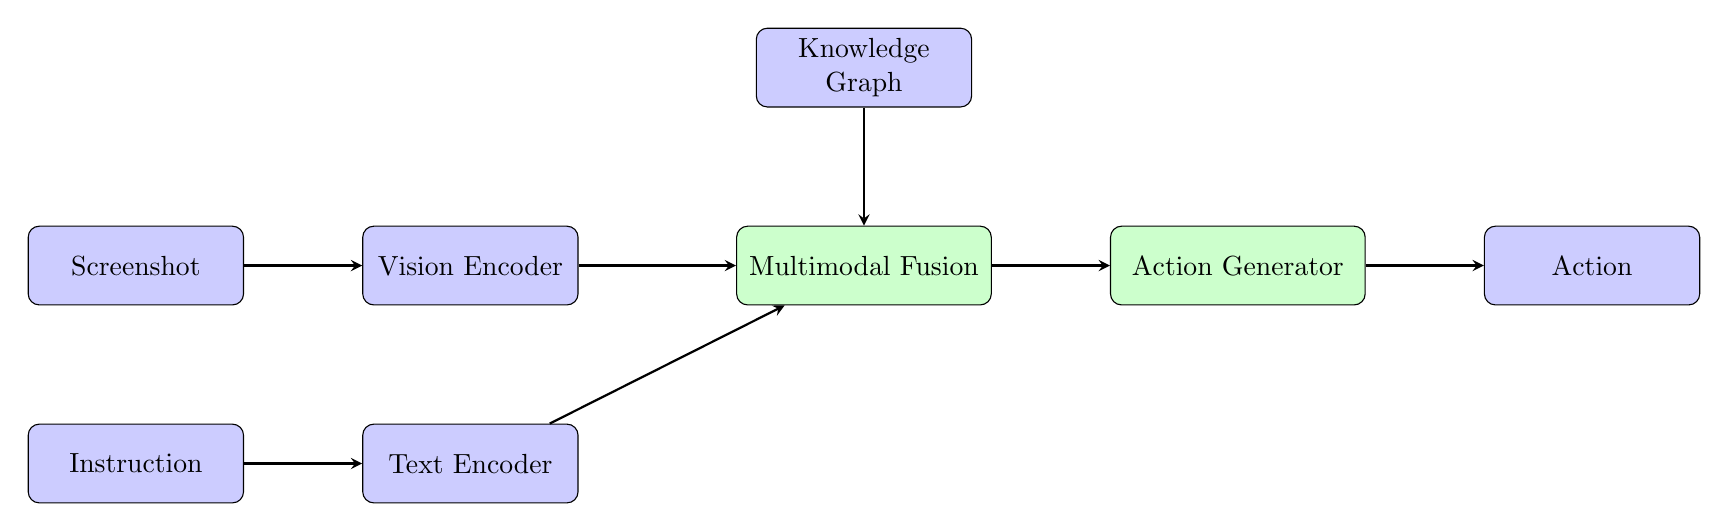
\begin{tikzpicture}[node distance=1.5cm, scale=1.0, transform shape]
\tikzstyle{block} = [rectangle, draw, fill=blue!20, text width=2.5cm, text centered, rounded corners, minimum height=1cm]
\tikzstyle{bigblock} = [rectangle, draw, fill=green!20, text width=3cm, text centered, rounded corners, minimum height=1cm]
\tikzstyle{arrow} = [thick,->,>=stealth]

\node[block] (img) {Screenshot};
\node[block, right=of img] (ve) {Vision Encoder};
\node[block, below=of img] (txt) {Instruction};
\node[block, right=of txt] (te) {Text Encoder};
\node[bigblock, right=2cm of ve] (fusion) {Multimodal Fusion};
\node[block, above=of fusion] (kg) {Knowledge Graph};
\node[bigblock, right=of fusion] (action) {Action Generator};
\node[block, right=of action] (output) {Action};

\draw[arrow] (img) -- (ve);
\draw[arrow] (txt) -- (te);
\draw[arrow] (ve) -- (fusion);
\draw[arrow] (te) -- (fusion);
\draw[arrow] (kg) -- (fusion);
\draw[arrow] (fusion) -- (action);
\draw[arrow] (action) -- (output);
\end{tikzpicture}
\caption{Unified framework architecture for knowledge-augmented GUI agents. The framework integrates visual perception, linguistic understanding, and structured knowledge through multimodal fusion to generate grounded actions.}
\label{fig:framework}
\end{figure}

\subsection{Vision Encoder Module}

The vision encoder should provide:

\begin{itemize}
    \item \textbf{High-resolution processing}: Preserve text and small icons.
    \item \textbf{Multi-scale features}: Capture both fine details and global layout.
    \item \textbf{OCR integration}: Extract text explicitly.
    \item \textbf{Element detection}: Identify interactive regions.
\end{itemize}

\subsection{Text Encoder Module}

The text encoder should provide:

\begin{itemize}
    \item \textbf{Instruction parsing}: Understand diverse command formats.
    \item \textbf{Semantic grounding}: Connect language to visual elements.
    \item \textbf{Knowledge retrieval}: Query external knowledge sources.
    \item \textbf{Multilingual support}: Enable cross-lingual transfer.
\end{itemize}

\subsection{Knowledge Graph Module}

The knowledge graph should encode:

\begin{itemize}
    \item \textbf{Element ontology}: Types and hierarchies of UI components.
    \item \textbf{Action models}: Preconditions, effects, and constraints.
    \item \textbf{Domain knowledge}: Application-specific semantics.
    \item \textbf{Commonsense}: General world knowledge for reasoning.
\end{itemize}

\subsection{Multimodal Fusion}

Fusion should integrate:

\begin{itemize}
    \item Visual features from the vision encoder.
    \item Textual embeddings from the text encoder.
    \item Structured knowledge from the knowledge graph.
    \item Dynamic state from interaction history.
\end{itemize}

Cross-modal attention mechanisms enable selective integration based on task requirements.

\subsection{Action Generation}

Action generation should produce:

\begin{itemize}
    \item Action type (click, type, scroll, etc.).
    \item Target specification (coordinates or element reference).
    \item Parameters (text to type, scroll direction, etc.).
    \item Confidence estimation for uncertainty handling.
\end{itemize}

\section{Future Research Directions}
\label{sec:future}

We identify promising directions for advancing knowledge-augmented GUI agents.

\subsection{Imbalanced Representation Learning}

Real-world UI datasets exhibit severe class imbalance:

\begin{itemize}
    \item Common elements (buttons, text) vastly outnumber rare elements (custom controls).
    \item Simple actions (click) dominate complex actions (drag-and-drop).
    \item Popular applications overshadow niche software.
\end{itemize}

Imbalanced representation learning techniques can address this:

\begin{itemize}
    \item \textbf{Focal loss}: Downweight easy examples during training.
    \item \textbf{Class-balanced sampling}: Oversample rare classes.
    \item \textbf{Curriculum learning}: Progress from common to rare cases.
    \item \textbf{Contrastive learning}: Learn discriminative features for minority classes.
\end{itemize}

\subsection{Prototype-Based Relation Modeling}

Prototype learning can improve element understanding:

\begin{enumerate}
    \item Learn prototype representations for element types (vision prototypes).
    \item Learn prototype representations for action types (text prototypes).
    \item Model relations between prototypes via attention or graph networks.
    \item Match observations to prototypes for classification and reasoning.
\end{enumerate}

This approach enables few-shot learning for novel element types and provides interpretable representations.

\subsection{Dynamic Knowledge Graph Evolution}

Static knowledge graphs become outdated as applications evolve. UI-Evol~\cite{uievol2024} demonstrates knowledge evolution through:

\begin{enumerate}
    \item \textbf{Retrace}: Reconstruct actual action sequences from screenshots.
    \item \textbf{Critique}: Compare observed behavior with expected knowledge.
    \item \textbf{Refine}: Update knowledge based on discrepancies.
\end{enumerate}

Future systems should:

\begin{itemize}
    \item Continuously update knowledge graphs from interaction logs.
    \item Detect knowledge conflicts and resolve them.
    \item Learn application-specific adaptations while preserving general knowledge.
\end{itemize}

\subsection{Neuro-Symbolic Integration}

Combining neural perception with symbolic reasoning offers:

\begin{itemize}
    \item \textbf{Explicit reasoning}: Interpretable derivation chains.
    \item \textbf{Constraint satisfaction}: Verifiable action validity.
    \item \textbf{Error diagnosis}: Traceable failure causes.
\end{itemize}

Promising approaches include:

\begin{itemize}
    \item Neural theorem proving for action planning.
    \item Differentiable logic programming for end-to-end training.
    \item LLM-guided symbolic reasoning for flexible inference.
\end{itemize}

\subsection{Multimodal Reasoning Chains}

Extending chain-of-thought reasoning to multimodal settings enables:

\begin{itemize}
    \item Explicit visual attention explanations.
    \item Step-by-step action justifications.
    \item Error detection and recovery.
\end{itemize}

Recent work on multimodal CoT shows promise but requires adaptation for GUI action generation.

\subsection{Safety and Alignment}

As GUI agents gain capabilities, safety becomes critical:

\begin{itemize}
    \item \textbf{Action filtering}: Prevent dangerous operations (deletion, system changes).
    \item \textbf{Permission systems}: Verify authorization before sensitive actions.
    \item \textbf{Rollback mechanisms}: Undo unintended changes.
    \item \textbf{Human oversight}: Confirmations for high-impact actions.
\end{itemize}

\section{Conclusion}
\label{sec:conclusion}

Graphical user interfaces pose unique challenges for artificial agents, requiring integration of visual perception, linguistic understanding, semantic reasoning, and sequential action planning. Human users overcome these challenges by leveraging rich world knowledge: we infer 3D structure from partial views, interpret polysemous icons through multiple knowledge sources, and rely on semantic memory for rapid comprehension.

This survey has demonstrated that existing vision-language models and agents often lack this knowledge, leading to hallucinations, brittle planning, and poor generalization. Through comprehensive review of cognitive foundations, vision encoders, text encoders, knowledge graphs, fusion architectures, benchmarks, and agents, we have established the importance of adopting semantic and world knowledge in GUI agents.

The proposed unified framework integrates four key components: high-resolution vision encoding for accurate perception, text encoding with linguistic knowledge for instruction understanding, knowledge graphs for structured semantic reasoning, and multimodal fusion for coherent integration. Future research should focus on imbalanced representation learning, prototype-based relation modeling, dynamic knowledge evolution, neuro-symbolic integration, and safety alignment.

Through continued efforts in these directions, we move closer to truly dependable and generalist computer use agents that can assist humans effectively across the full range of software applications.

\begin{thebibliography}{99}

\bibitem{slater1985}
Slater, A., Morrison, V., \& Rose, D. (1985).
Movement perception and identity constancy in the new-born baby.
\textit{British Journal of Developmental Psychology}, 3(3), 211--220.

\bibitem{soska2010}
Soska, K. C., \& Johnson, S. P. (2010).
Development of three-dimensional object completion in infancy.
\textit{Child Development}, 81(5), 1390--1404.

\bibitem{dessus2000}
Dessus, P., \& Peraya, D. (2000).
What are icons for? Cognitive load and learning from multimedia.
\textit{Computers in Human Behavior}, 16(3), 321--337.

\bibitem{sweller1988}
Sweller, J. (1988).
Cognitive load during problem solving: Effects on learning.
\textit{Cognitive Science}, 12(2), 257--285.

\bibitem{iconcomplex2020}
McDougall, S., \& Reppa, I. (2020).
Semantic complexity in icon comprehension.
\textit{Quarterly Journal of Experimental Psychology}, 73(7), 1039--1052.

\bibitem{rico2017}
Deka, B., et al. (2017).
Rico: A Mobile App Dataset for Building Data-Driven Design Applications.
\textit{ACM UIST}, 845--854.

\bibitem{dosovitskiy2020}
Dosovitskiy, A., et al. (2020).
An Image is Worth 16x16 Words: Transformers for Image Recognition at Scale.
\textit{ICLR 2021}.

\bibitem{cogagent2023}
Hong, W., et al. (2023).
CogAgent: A Visual Language Model for GUI Agents.
\textit{arXiv:2312.08914}.

\bibitem{omniparser2024}
Lu, Y., et al. (2024).
OmniParser for Pure Vision Based GUI Agent.
\textit{arXiv:2408.00203}.

\bibitem{showui2024}
Lin, K., et al. (2024).
ShowUI: One Vision-Language-Action Model for GUI Visual Agent.
\textit{arXiv:2411.17465}.

\bibitem{clip2021}
Radford, A., et al. (2021).
Learning Transferable Visual Models From Natural Language Supervision.
\textit{ICML 2021}.

\bibitem{llava2023}
Liu, H., et al. (2023).
Visual Instruction Tuning.
\textit{NeurIPS 2023}.

\bibitem{mrmkg2024}
Lee, S., et al. (2024).
Multimodal Reasoning with Multimodal Knowledge Graphs.
\textit{arXiv preprint}.

\bibitem{wkm2024}
Shah, R., et al. (2024).
World Knowledge Model for GUI Agents.
\textit{arXiv preprint}.

\bibitem{guiknowledgebench2024}
Liu, Y., et al. (2024).
GUI Knowledge Bench: Evaluating GUI Understanding in Multimodal Models.
\textit{arXiv:2406.10774}.

\bibitem{guiworld2024}
Chen, D., et al. (2024).
GUI-World: A Dataset for GUI-Oriented Multimodal LLM-based Agents.
\textit{arXiv:2406.10819}.

\bibitem{mind2web2023}
Deng, X., et al. (2023).
Mind2Web: Towards a Generalist Agent for the Web.
\textit{NeurIPS 2023}.

\bibitem{webarena2024}
Zhou, S., et al. (2024).
WebArena: A Realistic Web Environment for Building Autonomous Agents.
\textit{ICLR 2024}.

\bibitem{osworld2024}
Xie, T., et al. (2024).
OSWorld: Benchmarking Multimodal Agents for Open-Ended Tasks in Real Computer Environments.
\textit{arXiv:2404.07972}.

\bibitem{omniact2024}
Kapoor, R., et al. (2024).
OmniACT: A Dataset and Benchmark for Enabling Multimodal Generalist Autonomous Agents.
\textit{arXiv:2402.17553}.

\bibitem{aitw2023}
Rawles, C., et al. (2023).
Android in the Wild: A Large-Scale Dataset for Android Device Control.
\textit{NeurIPS 2023}.

\bibitem{androidcontrol2024}
Li, Y., et al. (2024).
AndroidControl: Enabling Automated UI Control of Android Devices.
\textit{arXiv preprint}.

\bibitem{ricosemantics2019}
Sunkara, M., et al. (2019).
Towards Building a Semantically Rich Dataset for Mobile UI Understanding.
\textit{arXiv preprint}.

\bibitem{iconqa2021}
Lu, P., et al. (2021).
IconQA: A New Benchmark for Abstract Diagram Understanding.
\textit{NeurIPS 2021}.

\bibitem{guicourse2024}
Chen, G., et al. (2024).
GUICourse: From General Vision Language Models to Versatile GUI Agents.
\textit{arXiv:2406.11317}.

\bibitem{webcog2024}
Zhang, Y., et al. (2024).
Web-CogDataset: A Cognitive Benchmark for Web Agents.
\textit{arXiv preprint}.

\bibitem{infiguiagent2024}
Liu, Z., et al. (2024).
InfiGUIAgent: A Multimodal Generalist GUI Agent with Native Reasoning.
\textit{arXiv:2412.18227}.

\bibitem{uitars2024}
Qin, Y., et al. (2024).
UI-TARS: Pioneering Automated GUI Interaction with Native Agents.
\textit{arXiv:2501.12326}.

\bibitem{seeclick2024}
Cheng, K., et al. (2024).
SeeClick: Harnessing GUI Grounding for Advanced Visual GUI Agents.
\textit{arXiv preprint}.

\bibitem{agents2024}
Wang, L., et al. (2024).
Agent S: An Open Agentic Framework that Uses Computers Like a Human.
\textit{arXiv:2410.08164}.

\bibitem{agents22025}
Wang, L., et al. (2025).
Agent S2: A Compositional Generalist GUI Agent.
\textit{arXiv preprint}.

\bibitem{claudecomputeruse2024}
Anthropic. (2024).
Introducing Computer Use.
\textit{Anthropic Blog}.

\bibitem{ariaui2024}
Yang, J., et al. (2024).
Aria-UI: Visual Grounding for GUI Instructions.
\textit{arXiv:2412.16256}.

\bibitem{uievol2024}
Wang, Y., et al. (2024).
UI-Evol: Bridging the Knowledge-Action Gap for GUI Agents.
\textit{arXiv preprint}.

\end{thebibliography}

\end{document}
